\documentclass{beamer}
\usetheme{metropolis}
\usepackage{graphicx}
\usepackage{amsmath}
\usepackage{tcolorbox}
\title{College Writing Seminar (INTD100): Week 1 Notes}
\author{Jordan Hanson}
\institute{Whittier College Department of Physics and Astronomy}

\begin{document}
\maketitle

\section{Summary}

\begin{frame}{Summary}
\begin{enumerate}
\item \textbf{Week 1}: \textit{Concise writing I:} In Week 1, we will focus on creating concise writing that eliminates extraneous words and sentences from your writing.
\begin{itemize}
\item Exercises: distilling complex scientific articles into shorter tracts of writing.
\item Exercises: reading popular scientific journal articles and discussing them in small groups
\item Exercises: Practice using analogies in communicating difficult or abstract scientific thoughts
\item Homeworks: Practice quotation and paraphrasing of experts in writing
\item Homeworks: practice descriptive detail by providing the reader with the correct details such that they understand something complex
\item Exploration topic: gravitational waves
\end{itemize}
\end{enumerate}
\end{frame}

\section{Introductions, Technology Check}

\begin{frame}{Introduction}
\begin{enumerate}
\item Professor Jordan Hanson (Physics and Astronomy)
\item Syllabus, journal
\item \alert{\textbf{Coggle.it}} accounts (mind-mapping and writing organization for concise writing)
\item Breakout rooms test
\item Simple exercise with Google Docs/Screenshare
\item \textbf{Summer reading assignment I}
\begin{itemize}
\item Discuss the essay by James Baldwin in breakout rooms
\item Discuss answers to exercises
\item Sort out logistical issues
\end{itemize}
\item Homework: read article regarding discovery of gravitational waves by the LIGO/Virgo collaborations
\item \alert{Theme for Module 1:} \textit{Keep it simple.}
\end{enumerate}
\end{frame}

\section{Summer Reading Assignment}

\begin{frame}{Summer Reading Assignment - Screen Share, Breakout Rooms}
\small
\begin{enumerate}
\item Create a Google Document in your shared Whittier College Google Drive. All first-year students should be
given a Google Drive shared space by Whittier College.
\item Create a enumerated list (1., 2., 3. etc.). Each item is to a separate mini-assignment, and each could take
between a few minutes and an hour.
\item Item 1: This essay is in a narrative style, and is broken into several parts. Summarize part I in one paragraph, using 120 words or fewer. Note: The purpose of this exercise is to complete the summary in no more than a
certain number of words. What key moments stand out in your mind? What is the central realization of the
author at the end of the section?
\item Item 2: Repeat exercise 1, but instead use only twenty words. What happens in part I of the essay?
\end{enumerate}
\end{frame}

\begin{frame}{Summer Reading Assignment - Screen Share, Breakout Rooms}
\small
\begin{enumerate}
\item Item 3: Consider part III. Construct a tract of writing that a) defines and explains the poison metaphor the
author describes at the funeral of his father, b) identifies the author’s “cure” or cures for the poison, and c)
provides several pieces of supporting evidence for the identification of the author’s cure.
\item Item 4: Consider the final part of the essay, when the author describes the fight in the Hotel Braddock. Write
a tract of between 200-400 words on the author’s treatment of evidence and facts. What does the author have
to say about the importance of facts about the fight to the people in that neighborbood? Notice the author’s
writing takes on the tone of a reporter regarding the ensuing riot. What facts stand out regarding the outcome?
\end{enumerate}
\end{frame}

\section{Homework Article 1}

\begin{frame}{LIGO Discovery of Gravitational Waves}
\textit{Homework article 1.0:} \\
\url{https://www.ligo.caltech.edu/news/ligo20160211} \\
\begin{itemize}
\item Please begin reading this article this week
\item We will use it for in-class exercises regarding concise writing and article-mapping
\end{itemize}
\end{frame}

\section{Concise Writing I: Use the eraser}

\begin{frame}{Concise Writing, 1}
How do we create concise writing?  Why is it important to be concise when writing for a scientific audience?
\begin{enumerate}
\item How...\textit{Be alone.}
\item How...\textit{Create an outline, mind-map or other plan}
\item How...\textit{\textbf{Use the eraser.}}  An eraser is a tool.  So is the delete button.
\item Why...Concise writing means fewer opportunities to be misunderstood
\item Why...Concise writing is easier to read
\item Why...Concise writing communicates abstract ideas into concrete form
\end{enumerate}
\end{frame}

\begin{frame}{Concise Writing, 1}
\textbf{Google Docs, Week 1}. \textit{Distill the following paragraph into a more conscise one.} \\ \vspace{0.25cm}
\textit{In order to measure the coefficient of friction of the rubber eraser, we placed the eraser on top of the plastic cover of the textbook and began to tilt it.  We continued to record the angle as we tilted the textbook.  Eventually, the eraser began to slide down the textbook.  We recorded that angle as well, and we calculated the tangent of that angle.  This was our first result for the coefficient of friction.  Next, we repeated the experiment many times and calculated an average coefficient of friction from the many trials.}
\alert{Pre-recorded content:} editing this down.
\end{frame}

\begin{frame}{Concise Writing, 1}
\textbf{Google Docs, Week 1}. \textit{Distill the following paragraph into a more conscise one.} \\ \vspace{0.25cm}
\textit{We set out to measure the specific heat of water by passing a wire through a bucket of water.  The water was 1000 milliliters and the water had a current of 2 amps.  The Joule heating equation tells us how many Joules of heat are produced in the wire which is radiated into the water.  We recorded the temperature of the water over time and recorded it next to the time in seconds.  We calcuated according to the Joule heating equation how many Joules per second was put into the water by the wire.  By comparing the rise in temperature of the water and the current we can calculate the conversion coefficient, which is the specific heat of water.}
\alert{Pre-recorded content:} editing this down.
\end{frame}

\section{Concise Writing II: Outlines and Mind-Maps}

\begin{frame}{Concise Writing II}
\begin{figure}
\centering
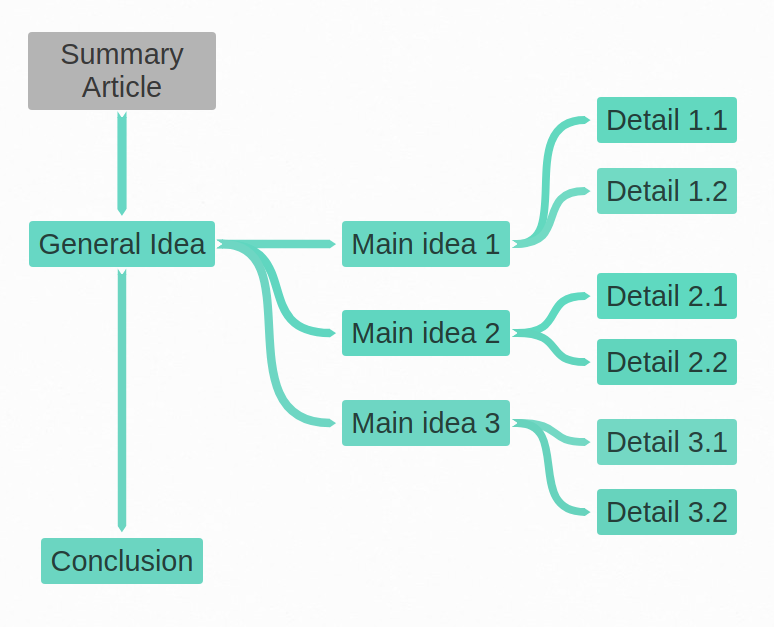
\includegraphics[width=0.7\textwidth]{figures/MindMap1.png}
\caption{\label{fig:mm1} A typical outline or mind-map for a scientific article for a wider audience.  For example, a summary of a field of research via Scientific American.}
\end{figure}
\end{frame}

\begin{frame}{Concise Writing II}
\begin{figure}
\centering
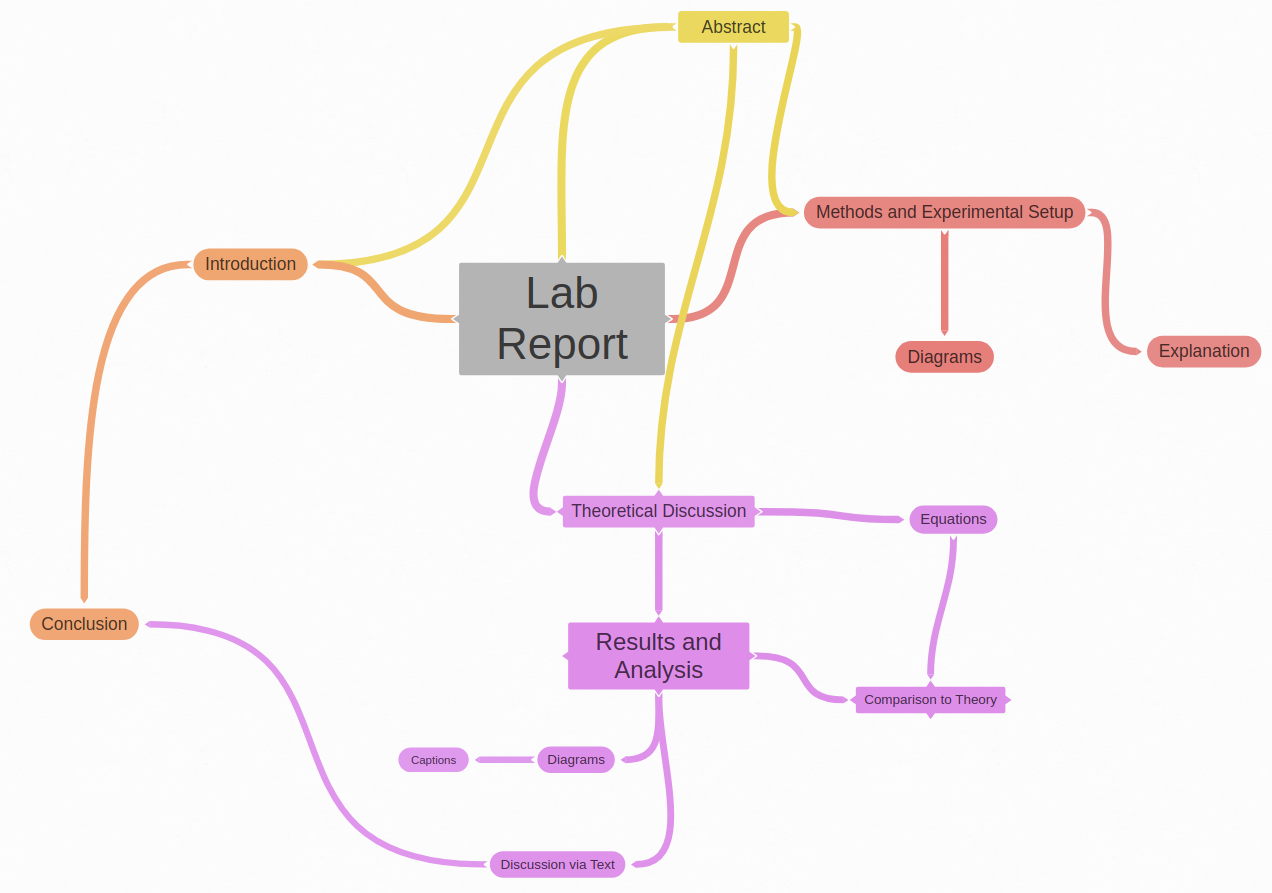
\includegraphics[width=0.75\textwidth]{figures/MindMap2.png}
\caption{\label{fig:mm2} A typical outline or mind-map for a college lab report with an abstract.}
\end{figure}
\end{frame}

\begin{frame}{Concise Writing II}
\begin{figure}
\centering
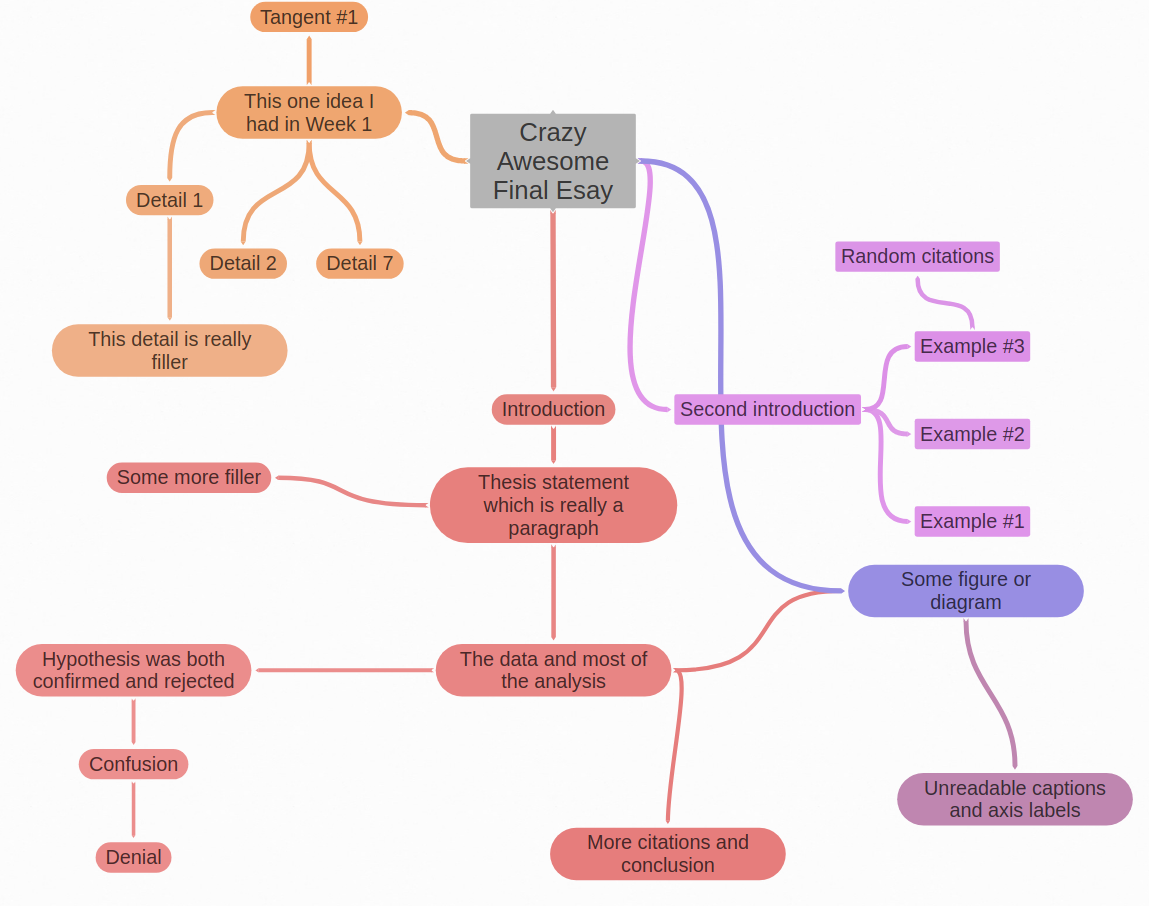
\includegraphics[width=0.75\textwidth]{figures/MindMap3.png}
\caption{\label{fig:mm3} What I often find in first-year essays in my physics courses.}
\end{figure}
\end{frame}

\begin{frame}{Concise Writing II}
\textbf{Coggle.it, Week 1}.
\begin{enumerate}
\item Write a $\approx 200$ word summary of what you read in the homework article.
\item Using Coggle.it, or the tool of your choice, create a mind-map or outline of the homework article regarding gravitational waves.
\item Think about your \textit{nodes} and \textit{connections}.  Is there a way to simplify the outline?
\item Write a $\approx 200$ word summary of what you read in the homework article, based on your outline or mind map.
\item Compare the two summaries.
\end{enumerate}
\end{frame}

\section{Concise Writing III}

\begin{frame}{Concise Writing III}
\small
Be alone. \\ \vspace{0.5cm}
\alert{\textbf{The essay on Moodle} Solitude and Leadership} by William Deresiewicz.
\end{frame}

\begin{frame}{Concise Writing III}
\begin{figure}
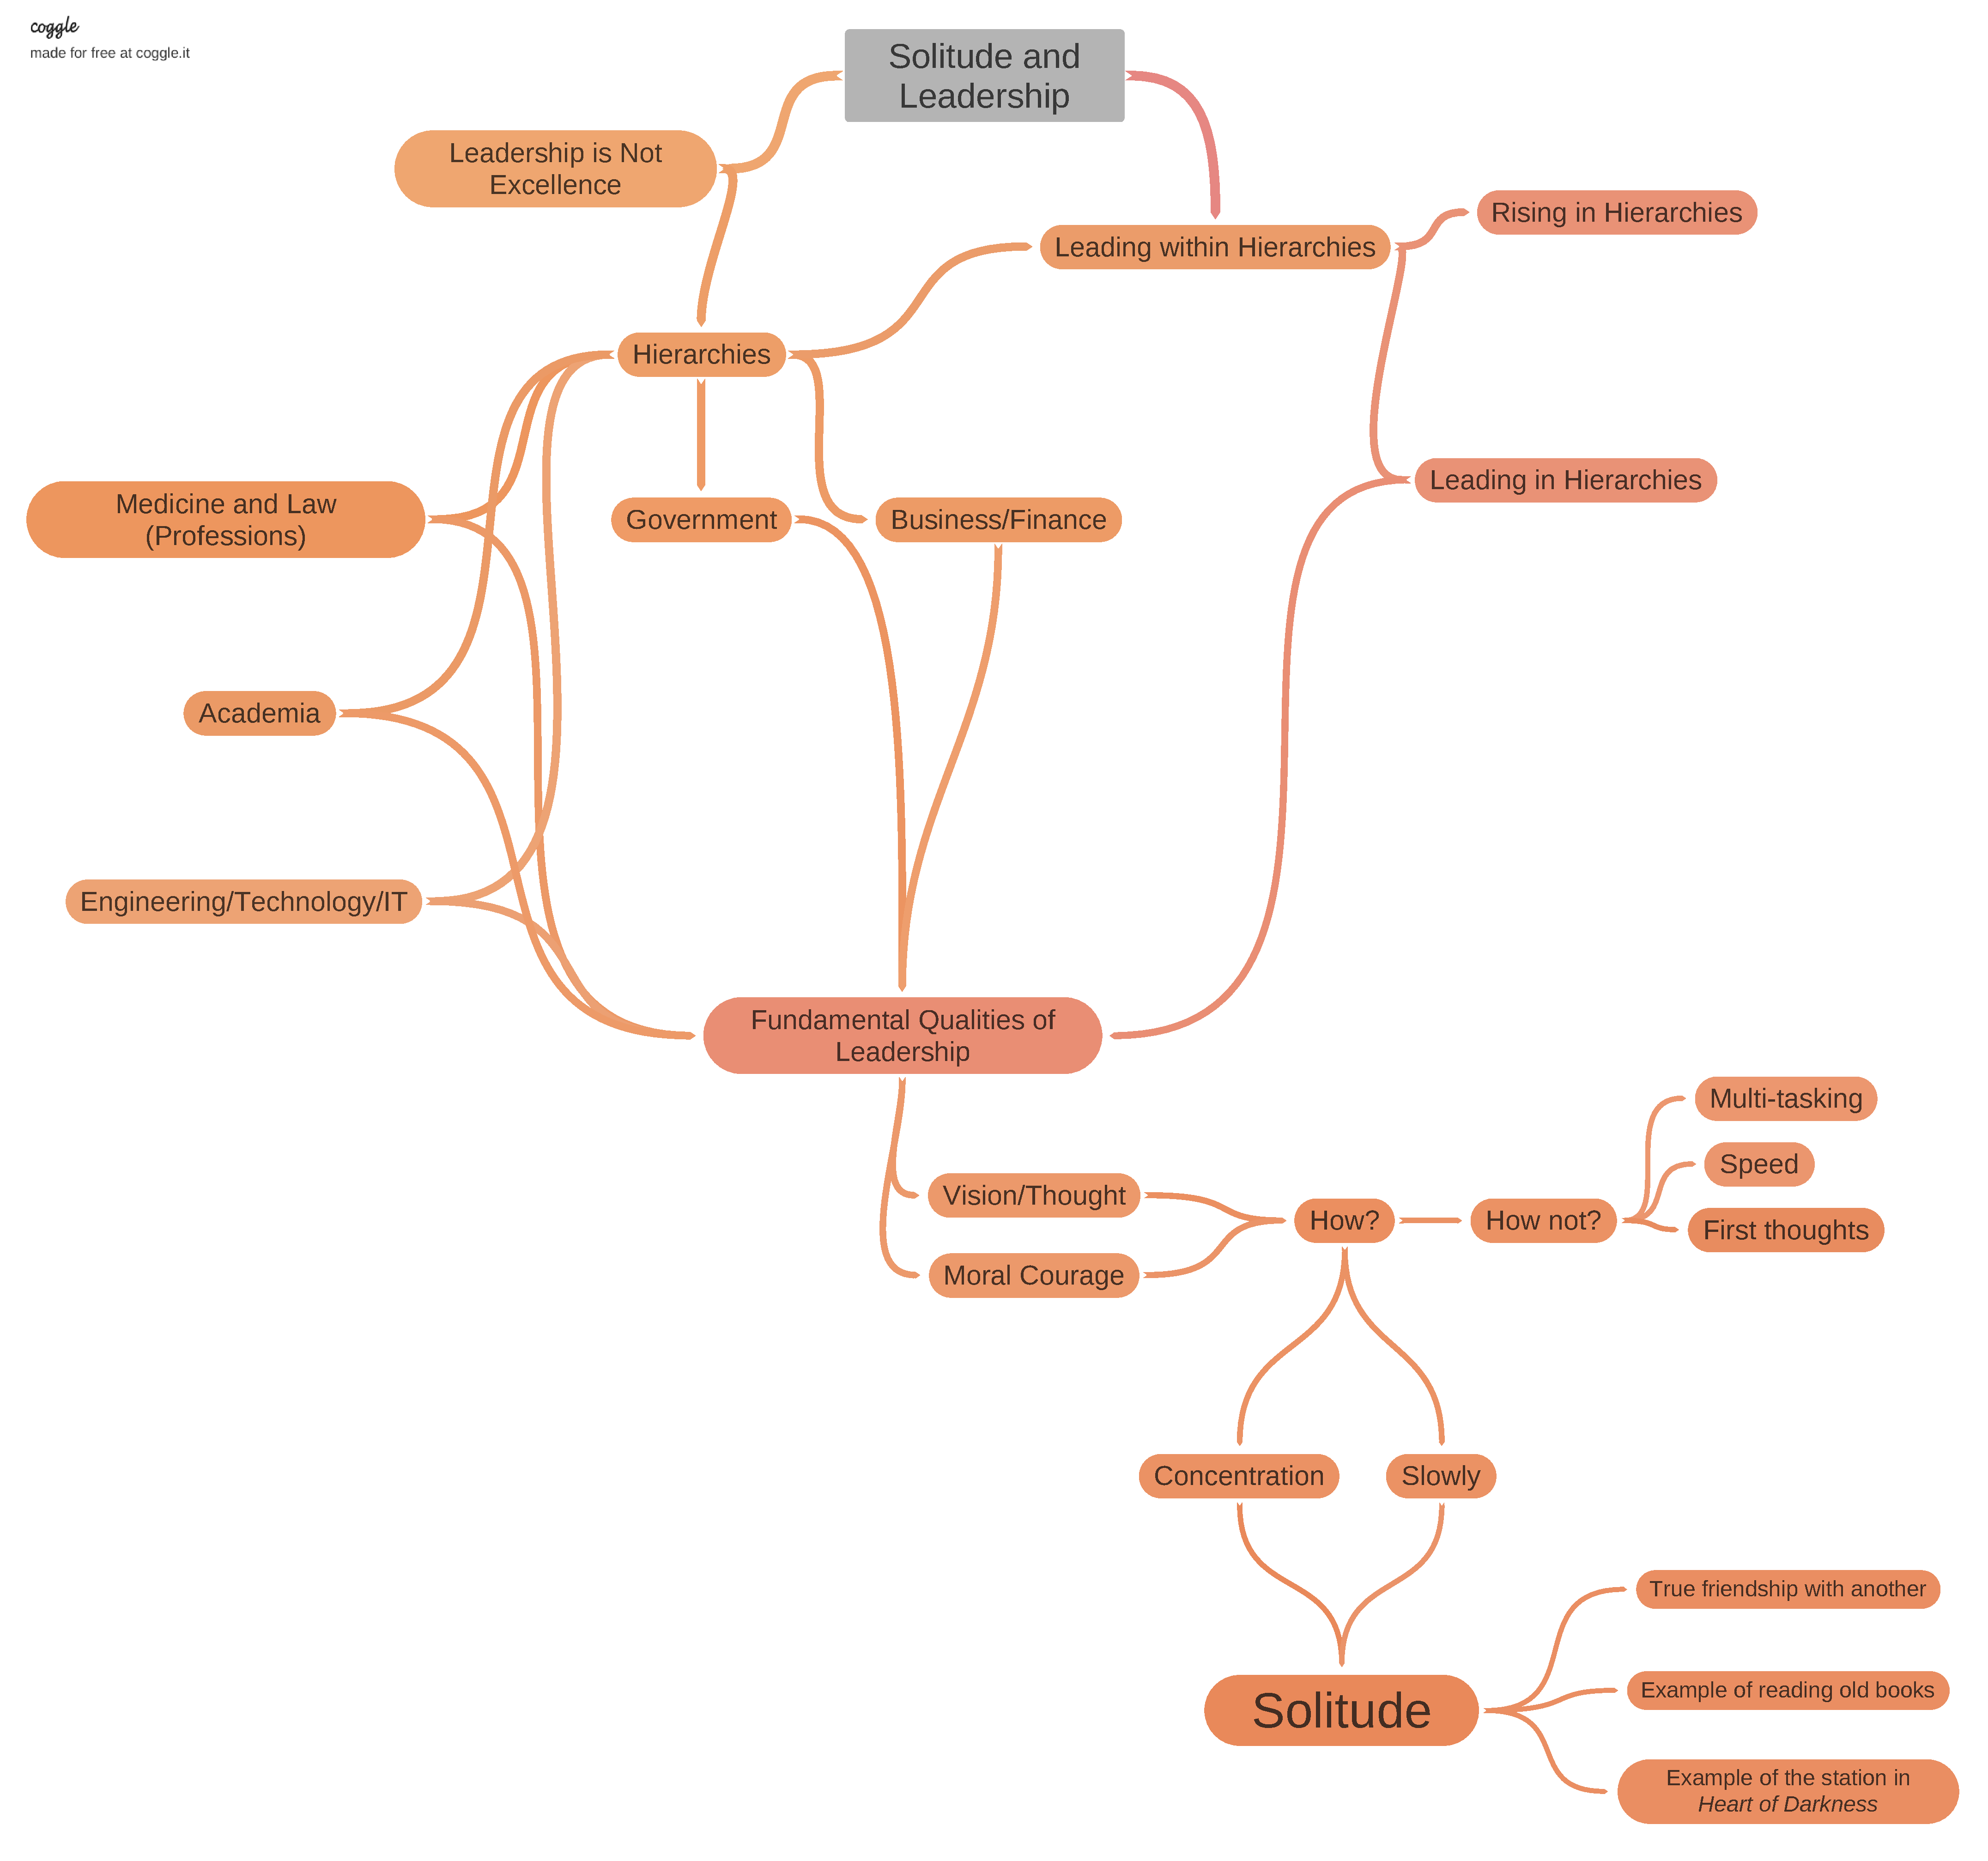
\includegraphics[width=0.7\textwidth]{figures/Solitude_and_Leadership.pdf}
\caption{\label{fig:leadership}  A map of the essay \textit{Solitude and Leadership.}}
\end{figure}
\end{frame}

\begin{frame}{Concise Writing III}
\begin{enumerate}
\item What is the central theme of the West Point article about leadership and solitude?
\item What does it mean to work alone in the context of leadership?  Leaders, by definition, are around other people.
\item Reflect on your writing \textit{process.}  If you cannot identify what process or processes you undertake to complete your writing, that's normal.  Write down a list of steps in your journal that constitute your writing process.
\end{enumerate}
\end{frame}

\begin{frame}{Concise Writing III}
\textbf{An example process: my own for longer reports.}
\begin{enumerate}
\item Make an outline, with enumeration and bullet points.
\item Walk away and think about something else
\item Re-do the outline, and ensure it has concrete goals and sub-goals.
\item \textit{Identify any important graphics or tables, and work on those first.}
\item Begin writing:
\begin{itemize}
\item Write the introduction first
\item Write the next section next, while cutting down the introduction
\item Write the third section next, while cutting down the second section...
\item Re-examine the whole structure periodically.
\end{itemize}
\end{enumerate}
\end{frame}

\section{Conclusion}

\begin{frame}{Summary}
\begin{enumerate}
\item \textbf{Week 1}: \textit{Concise writing I:} In Week 1, we will focus on creating concise writing that eliminates extraneous words and sentences from your writing.
\begin{itemize}
\item Exercises: distilling complex scientific articles into shorter tracts of writing.
\item Exercises: reading popular scientific journal articles and discussing them in small groups
\item Exercises: Practice using analogies in communicating difficult or abstract scientific thoughts
\item Homeworks: Practice quotation and paraphrasing of experts in writing
\item Homeworks: practice descriptive detail by providing the reader with the correct details such that they understand something complex
\item Exploration topic: gravitational waves
\end{itemize}
\end{enumerate}
\end{frame}

\end{document}
